% ==========================================================
% ENTREGA 1 — A pergunta do trabalho
% Teoria do Aprendizado Estatístico — Ciências de Dados
% Fatec Baixada Santista – Rubens Lara
% Derivado de modelo-trabalho.Rnw (R + knitr + abnTeX2)
% ==========================================================

\documentclass[
  article,
  12pt,
  oneside,
  a4paper,
  english,
  brazil
]{abntex2}\usepackage[]{graphicx}\usepackage[]{xcolor}
% maxwidth is the original width if it is less than linewidth
% otherwise use linewidth (to make sure the graphics do not exceed the margin)
\makeatletter
\def\maxwidth{ %
  \ifdim\Gin@nat@width>\linewidth
    \linewidth
  \else
    \Gin@nat@width
  \fi
}
\makeatother

\definecolor{fgcolor}{rgb}{0.345, 0.345, 0.345}
\newcommand{\hlnum}[1]{\textcolor[rgb]{0.686,0.059,0.569}{#1}}%
\newcommand{\hlsng}[1]{\textcolor[rgb]{0.192,0.494,0.8}{#1}}%
\newcommand{\hlcom}[1]{\textcolor[rgb]{0.678,0.584,0.686}{\textit{#1}}}%
\newcommand{\hlopt}[1]{\textcolor[rgb]{0,0,0}{#1}}%
\newcommand{\hldef}[1]{\textcolor[rgb]{0.345,0.345,0.345}{#1}}%
\newcommand{\hlkwa}[1]{\textcolor[rgb]{0.161,0.373,0.58}{\textbf{#1}}}%
\newcommand{\hlkwb}[1]{\textcolor[rgb]{0.69,0.353,0.396}{#1}}%
\newcommand{\hlkwc}[1]{\textcolor[rgb]{0.333,0.667,0.333}{#1}}%
\newcommand{\hlkwd}[1]{\textcolor[rgb]{0.737,0.353,0.396}{\textbf{#1}}}%
\let\hlipl\hlkwb

\usepackage{framed}
\makeatletter
\newenvironment{kframe}{%
 \def\at@end@of@kframe{}%
 \ifinner\ifhmode%
  \def\at@end@of@kframe{\end{minipage}}%
  \begin{minipage}{\columnwidth}%
 \fi\fi%
 \def\FrameCommand##1{\hskip\@totalleftmargin \hskip-\fboxsep
 \colorbox{shadecolor}{##1}\hskip-\fboxsep
     % There is no \\@totalrightmargin, so:
     \hskip-\linewidth \hskip-\@totalleftmargin \hskip\columnwidth}%
 \MakeFramed {\advance\hsize-\width
   \@totalleftmargin\z@ \linewidth\hsize
   \@setminipage}}%
 {\par\unskip\endMakeFramed%
 \at@end@of@kframe}
\makeatother

\definecolor{shadecolor}{rgb}{.97, .97, .97}
\definecolor{messagecolor}{rgb}{0, 0, 0}
\definecolor{warningcolor}{rgb}{1, 0, 1}
\definecolor{errorcolor}{rgb}{1, 0, 0}
\newenvironment{knitrout}{}{} % an empty environment to be redefined in TeX

\usepackage{amsmath}
\usepackage{alltt}

\usepackage[T1]{fontenc}
\usepackage[utf8]{inputenc}
\usepackage{lmodern}
\usepackage{amsmath,amssymb}
\usepackage{icomma}
\usepackage{booktabs}
\usepackage{enumitem}
\usepackage[alf]{abntex2cite}

\setlist{noitemsep, topsep=3pt, parsep=1pt, partopsep=0pt}
\setlength{\parskip}{0.35em}

\hypersetup{hidelinks}

% ----------------------------------------------------------
% DADOS DA ENTREGA
% ----------------------------------------------------------
\titulo{A pergunta do trabalho: Fatores Associados à Concentração de Sinistros de Trânsito nos Horários de Pico}
\tituloestrangeiro{}
\autor{Grupo APPA}
\local{Santos-SP}
\data{\today}

\newcommand{\nomecurso}{Tecnologia em Ciência de Dados}
\newcommand{\nomedisciplina}{Teoria do Aprendizado Estatístico}
\newcommand{\nomeprofessor}{Prof.\ Dr.\ João Paulo Ferreira de Mello}
\newcommand{\repositorio}{https://github.com/kyl8/aprendizado-estatistico}
\newcommand{\integrantes}{%
  Arthur Galvão \\
  Pedro Henrique \\
  Pedro Alvarenga \\
  Ailana%
}
\IfFileExists{upquote.sty}{\usepackage{upquote}}{}
\begin{document}





\selectlanguage{brazil}
\frenchspacing

% ----------------------------------------------------------
% IDENTIFICAÇÃO
% ----------------------------------------------------------
\maketitle

\begin{center}
  \footnotesize
  Fatec Baixada Santista -- Rubens Lara \quad|\quad
  \nomecurso{} \quad|\quad \nomedisciplina{} \\[0.2em]
  \nomeprofessor{} \quad|\quad Repositório: \texttt{\repositorio} \\[0.2em]
  \textbf{Integrantes:} \integrantes
\end{center}

\textual

% ==========================================================================
\section{Introdução}
% ==========================================================================

Os sinistros de trânsito são um problema frequente nas cidades, principalmente nos horários de pico, quando há maior circulação de veículos e pessoas. O aumento do fluxo pode favorecer congestionamentos, frenagens e conflitos no trânsito. Este trabalho apresenta o banco de dados escolhido, formula a pergunta sobre a maior ocorrência de sinistros nos horários de pico e verifica se os dados permitem respondê-la. Para isso, serão analisados os registros de sinistros, considerando seus horários e outras características disponíveis no banco de dados. A análise busca identificar padrões e possíveis fatores relacionados à maior frequência de ocorrências nesses períodos. Assim, a pergunta central é: \textbf{por que os sinistros de trânsito acontecem com mais frequência nos horários de pico?}

Em segurança viária e mobilidade urbana, compreender os mecanismos subjacentes a essa concentração temporal é imprescindível para órgãos de planejamento de tráfego, secretarias municipais e operadoras de rodovias. A literatura de tráfego aponta que o aumento de sinistros nesses períodos decorre da combinação entre saturação da malha viária, redução do intervalo de seguimento (\textit{headway}) entre veículos, atrito entre modais heterogêneos (veículos pesados, motocicletas e pedestres) e pressões temporais dos deslocamentos pendulares. Sob o arcabouço de Teoria do Aprendizado Estatístico \cite{james2021}, o estudo adota uma abordagem inferencial fundamentada em modelos supervisionados de classificação, quantificando o efeito marginal dos fatores operacionais e viários que caracterizam os episódios ocorridos no pico em relação aos demais turnos.

% ==========================================================================
\section{O banco de dados e o problema}
% ==========================================================================

O conjunto de dados foi extraído do repositório oficial do Infosiga SP \cite{fonte_dados}, gerido pelo Departamento Estadual de Trânsito de São Paulo (Detran-SP), abrangendo as ocorrências registradas entre janeiro de 2025 e junho de 2026. A base consolida dados de boletins policiais e notificações viárias em todo o território estadual. Conforme preconiza a norma técnica da Associação Brasileira de Normas Técnicas para pesquisa viária \cite{abnt10697}, adota-se rigorosamente a denominação ``sinistro de trânsito'', superando o termo coloquial ``acidente''.

Cada linha da base representa uma ocorrência única de sinistro de trânsito devidamente registrada por boletim de ocorrência policial. Foram selecionados os boletins com horário de ocorrência válido, totalizando $n = \text{151591}$ observações e $p = \text{12}$ preditores candidatos. As variáveis contemplam atributos de infraestrutura (\texttt{tipo\_via}), características do evento (\texttt{tp\_sinistro\_primario}), temporalidade (\texttt{dia\_da\_semana}, \texttt{turno}), gravidade (\texttt{fatal}) e a contagem discriminada de modais envolvidos (\texttt{qtd\_automovel}, \texttt{qtd\_motocicleta}, \texttt{qtd\_onibus}, \texttt{qtd\_caminhao}, \texttt{qtd\_pedestre}, \texttt{qtd\_bicicleta} e total de \texttt{veiculos}).

A escolha deste banco fundamenta-se na alta completude cadastral dos boletins policiais e na relevância concreta do problema: gestores de mobilidade e comandos de policiamento viário necessitam de evidências quantitativas para priorizar intervenções de engenharia de tráfego, temporização semafórica dinâmica e patrulhamento preventivo nos corredores de maior atrito.

% ==========================================================================
\section{A pergunta}
% ==========================================================================

A pergunta norteadora da pesquisa é enunciada de forma direta: \textbf{por que os sinistros de trânsito acontecem com mais frequência nos horários de pico?} A Tabela~\ref{tab:ficha} sintetiza os sete campos metodológicos que estruturam formalmente a investigação.

\begin{table}[htb]
  \centering
  \caption{Ficha da pergunta}
  \label{tab:ficha}
  \footnotesize
  \begin{tabular}{@{}p{0.32\textwidth}p{0.62\textwidth}@{}}
    \toprule
    \textbf{Campo} & \textbf{Preenchimento} \\
    \midrule
    1. A pergunta, em uma frase & Por que os sinistros de trânsito acontecem com mais frequência nos horários de pico? \\
    2. Resposta $Y$: coluna, tipo & \texttt{pico} --- qualitativa (binária: Pico vs.\ Fora do Pico) \\
    3. Preditores $X$: quais e quantos & Vias, tipo de colisão, modais envolvidos, dia da semana e severidade ($p = \text{12}$) \\
    4. Tipo: decisões de modelagem & Supervisionado; classifica\c{c}\~ao; abordagem inferencial \\
    5. Métrica de avaliação & acur\'acia e AUC \\
    6. Linha de base a bater & acur\'acia = 0,599 \quad (chutar a classe mais comum) \\
    7. Dono do problema & Órgãos de trânsito e prefeituras (alocação de efetivo e intervenções semafóricas) \\
    \bottomrule
  \end{tabular}
  \fonte{Elaborada pelos autores.}
\end{table}

A decisão por um problema de \textbf{classificação supervisionada com finalidade inferencial} é metodologicamente determinante. Conforme discutido por \citeonline{bruce2019}, em ciências aplicadas o objetivo não é meramente prever se um sinistro futuro pertencerá ao pico, mas identificar e mensurar as razões de chance (\textit{odds ratios}) de cada fator de risco. Modelos lineares generalizados (regressão logística com inferência assintótica e reamostragem via validação cruzada) permitem isolar o impacto marginal de conflitos entre motocicletas e automóveis em vias arteriais, fornecendo suporte acionável para políticas públicas de redução de sinistralidade.

% ==========================================================================
\section{Defesa da pergunta}
% ==========================================================================

A Tabela~\ref{tab:diag} consolida o diagnóstico empírico realizado sobre o banco de dados.

\begin{table}[htb]
  \centering
  \caption{Diagnóstico do banco}
  \label{tab:diag}
  \footnotesize
  \begin{tabular}{@{}p{0.34\textwidth}p{0.60\textwidth}@{}}
    \toprule
    \textbf{Verificação} & \textbf{Resultado} \\
    \midrule
    Tamanho ($n \times p$)   & $\text{151591} \times \text{12}$ observações e preditores \\
    Linha de base            & acur\'acia = 0,599 \quad (chutar a classe mais comum) \\
    Maior correlação com $Y$ & n\~ao se aplica (resposta qualitativa) \\
    Balanço das classes      & \texttt{Fora do Pico}: 90743 | \texttt{Pico}: 60848 \\
    Valores faltantes        & nenhum \\
    \bottomrule
  \end{tabular}
  \fonte{Elaborada pelos autores.}
\end{table}

\textbf{Vazamento.} Para evitar contaminação do modelo, as variáveis que definiam a hora original de registro (\texttt{hora\_sinistro}) foram completamente desconsideradas do conjunto de preditores $X$. Dessa forma, a classificação opera estritamente sobre características ambientais, viárias e estruturais do sinistro, garantindo que o modelo capture a assinatura comportamental do tráfego no pico sem vazamento de informação trivial.

\textbf{Tamanho ($n \times p$).} O conjunto reúne $n = \text{151591}$ observações para $p = \text{12}$ preditores candidatos. A relação de mais de 12.000 observações por parâmetro assegura ampla estabilidade aos estimadores de máxima verossimilhança, eliminando riscos de sobreajuste (\textit{overfitting}) e permitindo a inclusão de termos de interação entre tipos de via e modais vulneráveis.

\textbf{Balanço de classes e faltantes.} A resposta qualitativa binária exibe excelente balanço entre as classes: 40,1\% das ocorrências concentram-se nas faixas de pico pendular (\text{NA} sinistros em apenas 6,5 horas do dia), enquanto 59,9\% distribuem-se nas 17,5 horas restantes (\text{NA} sinistros). A Figura~\ref{fig:resposta} ilustra essa distribuição. Adicionalmente, o subconjunto de boletins selecionados não apresenta valores faltantes (\texttt{NA}) nas variáveis incluídas na modelagem.

\begin{figure}[htb]
  \centering
  \caption{Distribuição da variável de resposta \texttt{pico}}
  \label{fig:resposta}
\begin{knitrout}
\definecolor{shadecolor}{rgb}{0.969, 0.969, 0.969}\color{fgcolor}

{\centering 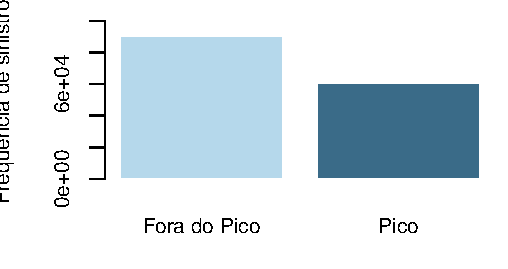
\includegraphics[width=0.38\linewidth]{figure/fig-resposta-1} 

}


\end{knitrout}
  \fonte{Elaborada pelos autores.}
\end{figure}

\textbf{Veredito.} A pergunta se sustenta plenamente nos dados: o banco possui volume massivo, integridade cadastral e atributos suficientes para explicar a dinâmica dos sinistros no horário de pico por meio de aprendizado estatístico inferencial. A modelagem detalhada será aprofundada nas próximas etapas do projeto através de regressão logística, seleção de preditores por regularização e reamostragem via validação cruzada e bootstrap.

% ----------------------------------------------------------
% REFERÊNCIAS
% ----------------------------------------------------------
\postextual
\bibliography{referencias}

\end{document}
